%!TEX root = ../../Main.tex
\graphicspath{{Chapters/System/}}
%-------------------------------------------------------------------------------


\section{System beskrivelse}
I dette afsnit laves et overblik over systemets blokke og de interne fobindelser. Derudover gives et overblik over funktionerne som er implementeret i projektet. 
På figur \ref{fig:Bdd} ses et overordnet Bdd for projektet, hvor de interne forbindelser forklares på figur \ref{fig:Ibd}. 

\begin{figure}[H]
	\centering
	\includegraphics[width = 500 pt]{Img/Bdd.png}
	\caption{Bdd af BA-TA}
	\label{fig:Bdd}
\end{figure}

\subsection{Blokbeskrivelse BA-TA}
I det følgende vil komme en beskrivelse af de enkelte blokke i BA-TA og deres interne funktionalitet.
\newline
\newline
\textbf{Arduino} \\*
Arduino står for at styre hele systemet. Den skal styre alt funktionalitet som projektet skal udføre, og står som master ift. resten af projektet. Arduino blokken står for at initialisere  controller blokkene, hhv. Touch og Display, derudover står den for at modtage signaler fra touch, og sende signaler til display. Derudover står den for at få bluetooth til at sende de respektive værdier.
\newline
\newline
\textbf{Touch Controller} \\*
Touch Controller står for at modtage værdier fra Touch Display, sende værdien videre til Arduino 
\newline
\newline
\textbf{Display Controller} \\*
Display Controller står for modtage en værdi fra Arduino og sende sende værdien til Touch Display. \newline
\newline
\textbf{Bluetooth} \\*
Er et bluetooth modul, som vha. AT kommandoer kan kommunikere med Arduino.
\newline
\newline
\textbf{Touch Display} \\*
Touch Display fungerer som brugergrænseflade og integering mellem system og bruger. 
\subsection{Internal Block Diagram for BA-TA}
På figur \ref{fig:Ibd} ses et overordnet IBD over selve systemet, som er bygget på Bdd'et. 
\begin{figure}[H]
	\centering
	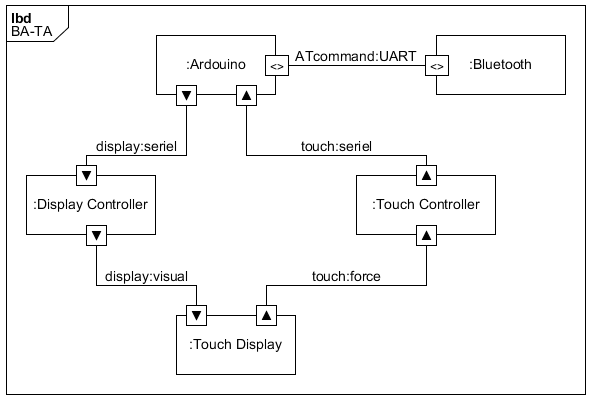
\includegraphics[width = 300 pt]{Img/Ibd.png}
	\caption{Ibd af BA-TA}
	\label{fig:Ibd}
\end{figure}

\subsection{Entity Relationship Diagram for BA-TA}
Herefter gives et overblik på figur \ref{fig:Entity} over koden til driverne som er skrevet til dette projekt. 

\begin{figure}[H]
	\centering
	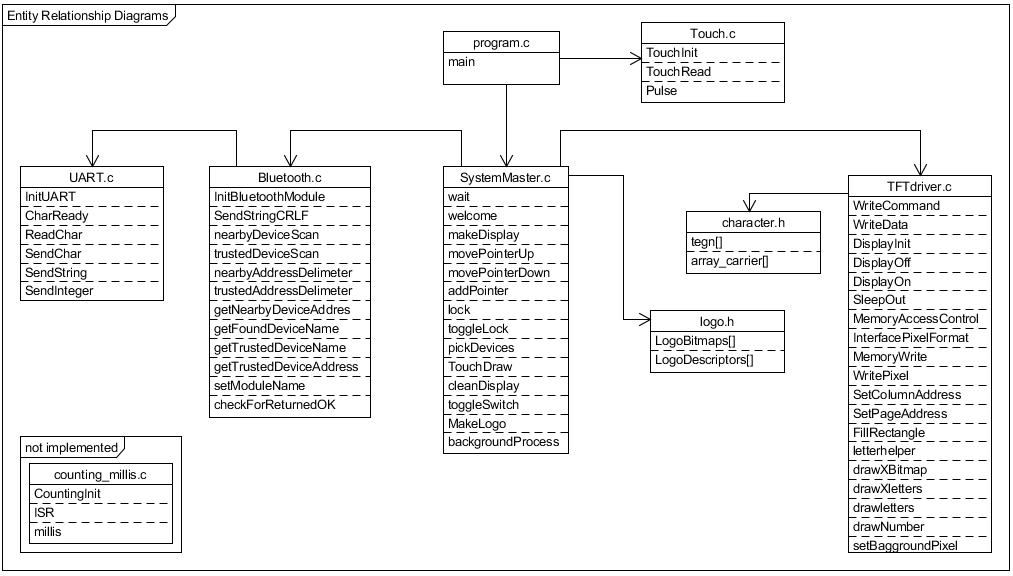
\includegraphics[width = 300 pt]{Img/Entity.png}
	\caption{Entity Relationship Diagrams}
	\label{fig:Entity}
\end{figure}

